% slides.tex: slide deck for the experiment brief (docs/brief.md), with its figures and tables in the same order.
% Build from the repo root:
%   latexmk -cd -lualatex -interaction=nonstopmode -outdir=../_build/slides docs/slides.tex
%   cp _build/slides/slides.pdf docs/slides.pdf
\documentclass[aspectratio=169,11pt]{beamer}
\usepackage{fontspec}
\setsansfont{OpenSans}[Extension=.ttf, UprightFont=*-Regular, BoldFont=*-Bold, ItalicFont=*-Italic,
                       BoldItalicFont=*-BoldItalic]
\usepackage{booktabs}
\usepackage{array}
\newcolumntype{L}[1]{>{\raggedright\arraybackslash}p{#1}}
\graphicspath{{../figs/}}

% Same colours as the brief (lapreprint blue theme).
\definecolor{brand}{HTML}{0E4B92}
\definecolor{accent}{HTML}{357ABF}
\definecolor{muted}{HTML}{6D6E70}
\setbeamercolor{normal text}{fg=black!85}
\setbeamercolor{structure}{fg=brand}
\setbeamercolor{title}{fg=brand}
\setbeamerfont{title}{size=\LARGE,series=\bfseries}
\setbeamertemplate{navigation symbols}{}
\setbeamertemplate{itemize items}[circle]
\setbeamertemplate{frametitle}{%
  \vspace{0.5em}{\color{accent}\scriptsize\bfseries\MakeUppercase{\insertframesubtitle}}\par
  {\color{brand}\large\bfseries\insertframetitle}\par\vspace{-0.2em}}
\setbeamertemplate{footline}{%
  \hspace{1.2em}{\color{muted}\tiny Pretrained audio models for noise detection}\hfill
  {\color{muted}\tiny\insertframenumber\,/\,\inserttotalframenumber}\hspace{1.2em}\vspace{0.8em}}

% \sidefig{kicker}{title}{figure file}{figure width}{notes width}{\item ... notes}
\newcommand{\sidefig}[6]{%
\begin{frame}{#2}\framesubtitle{#1}
  \begin{columns}[c,onlytextwidth]
    \begin{column}{#4\textwidth}\centering
      \includegraphics[width=\linewidth,height=0.8\textheight,keepaspectratio]{#3}
    \end{column}
    \begin{column}{#5\textwidth}\small
      \begin{itemize}\setlength{\itemsep}{0.7em}#6\end{itemize}
    \end{column}
  \end{columns}
\end{frame}}

\title{Transferring pretrained audio models to artificial noise and abiotic sound}
\subtitle{Experiment brief}
\author{Amy Van Scoyoc}
\institute{UC Berkeley}
\date{\today}

\begin{document}

\begin{frame}[plain]
  \vfill\titlepage\vfill
\end{frame}

\begin{frame}{Do frozen pretrained audio models transfer to noise in ARU data?}\framesubtitle{Overview}
  \begin{itemize}\setlength{\itemsep}{0.6em}
    \item \textbf{Classes:} 14 target classes in ARU recordings, 11 artificial and 3 abiotic; 9 animal and other
          classes serve only as negatives
    \item \textbf{Models:} BirdNET 2.4, BirdNET 3.0, Perch v8 and Perch 2.0 (bird); CNN14 (AudioSet);
          ResNet-18 (ImageNet), all frozen
    \item \textbf{Adaptation:} a small MLP head on the embeddings, trained on N = 5--160 clips per class, with
          10 random training draws per N
    \item \textbf{Test:} 50 clips per class from recordings never used for training
    \item \textbf{Zero-shot:} the model's own label for the class, where one exists
  \end{itemize}
\end{frame}

\begin{frame}{Fourteen noise classes, split by source recording}\framesubtitle{Table 1 \textperiodcentered{} Data}
  \centering\scriptsize
  \begin{tabular}{llrrrr}
    \toprule
    Class & Type & Recordings / clips & Test rec. / clips & Training rec. / clips & Max N \\
    \midrule
    Device static & artificial & 168 / 1,416 & 9 / 50 & 159 / 1,366 & 160 \\
    Generator & artificial & 32 / 437 & 10 / 50 & 22 / 384 & 160 \\
    Traffic & artificial & 53 / 297 & 13 / 50 & 40 / 242 & 160 \\
    Engine & artificial & 115 / 170 & 38 / 50 & 76 / 117 & 80 \\
    Power tools & artificial & 11 / 162 & 9 / 29 & 2 / 133 & 80 \\
    Human vocal & artificial & 16 / 117 & 14 / 50 & 2 / 64 & 40 \\
    Metal clanging * & artificial & 28 / 60 & 13 / 30 & 15 / 30 & 20 \\
    Airplane * & artificial & 12 / 52 & 6 / 25 & 6 / 27 & 20 \\
    Gun * & artificial & 7 / 19 & 5 / 9 & 2 / 10 & 10 \\
    Fireworks * & artificial & 4 / 13 & 2 / 6 & 2 / 7 & 5 \\
    Human non-vocal * & artificial & 2 / 8 & 1 / 3 & 1 / 5 & 5 \\
    Wind & abiotic & 106 / 508 & 11 / 50 & 94 / 453 & 160 \\
    Thunder * & abiotic & 5 / 21 & 2 / 8 & 3 / 13 & 10 \\
    Water * & abiotic & 3 / 11 & 2 / 5 & 1 / 6 & 5 \\
    \bottomrule
  \end{tabular}\par\vspace{0.4em}
  {\color{muted}* Low-sample class (fewer than 90 clips; provisional).\quad
   Power tools and human vocal have only 2 training recordings each.}
\end{frame}

\sidefig{Figure 1 \textperiodcentered{} How many clips?}{Performance levels off near N = 40 for most classes}
  {saturation_main.pdf}{0.55}{0.42}{%
  \item Most curves come within 0.02 AUC of their best by N = 40
  \item Device static and traffic are still rising at N = 160
  \item Going from 40 to 80 clips adds 0.01--0.04 AUC
  \item Open markers at N = 0: the model's own label (zero-shot)}

\sidefig{Figure 2 \textperiodcentered{} Summary at N = 40}{The class matters more than the model}
  {saturation_summary.pdf}{0.5}{0.47}{%
  \item Class means range from 0.97 (wind) to 0.69 (power tools)
  \item Model means range from 0.78 (BirdNET 3.0) to 0.87 (BirdNET 2.4)
  \item The trained head beats the built-in label in 13 of 29 known pairs (median N = 5)
  \item No model has a label for generator}

\sidefig{Figure 3 \textperiodcentered{} Cross-detection}{Binary detectors respond to similar noise}
  {cross_detection.pdf}{0.7}{0.27}{%
  \item Detected = $p \geq 0.5$; diagonal = recall
  \item Mean recall 0.55--0.62; false alarms 0.14--0.23
  \item Groups: impulsive sounds, wind and thunder, vehicles}

\sidefig{Figure 4 \textperiodcentered{} Multiclass}{One head recognises wind, not generator or power tools}
  {confusion_matrices_noise.pdf}{0.68}{0.29}{%
  \item 7 classes with $\geq$ 40 training clips
  \item Wind recall 0.90--0.97
  \item Generator and power tools 0.13--0.32, mostly called traffic or engine
  \item Device static is often called wind
  \item Macro F1 0.43--0.55}

\sidefig{Figure 5 \textperiodcentered{} Embeddings}{The confusions are already in the embeddings}
  {tsne_embeddings_noise.pdf}{0.68}{0.29}{%
  \item t-SNE of raw test-clip embeddings; no classifier
  \item Device static is compact in most models
  \item Generator, traffic, engine and power tools overlap}

\sidefig{Figure 6 \textperiodcentered{} Binary vs multiclass}{Both discriminate each class about equally well}
  {binary_vs_multiclass_auc_noise.pdf}{0.62}{0.35}{%
  \item Same 40 training clips and the same positive test clips
  \item Mean difference $-0.002$ (range $-0.14$ to $+0.10$)
  \item Largest drop: device static, for which wind is a hard negative}

\begin{frame}{Longer input windows help only generator}\framesubtitle{Figure 7 \textperiodcentered{} BirdNET 3.0 window length}
  \centering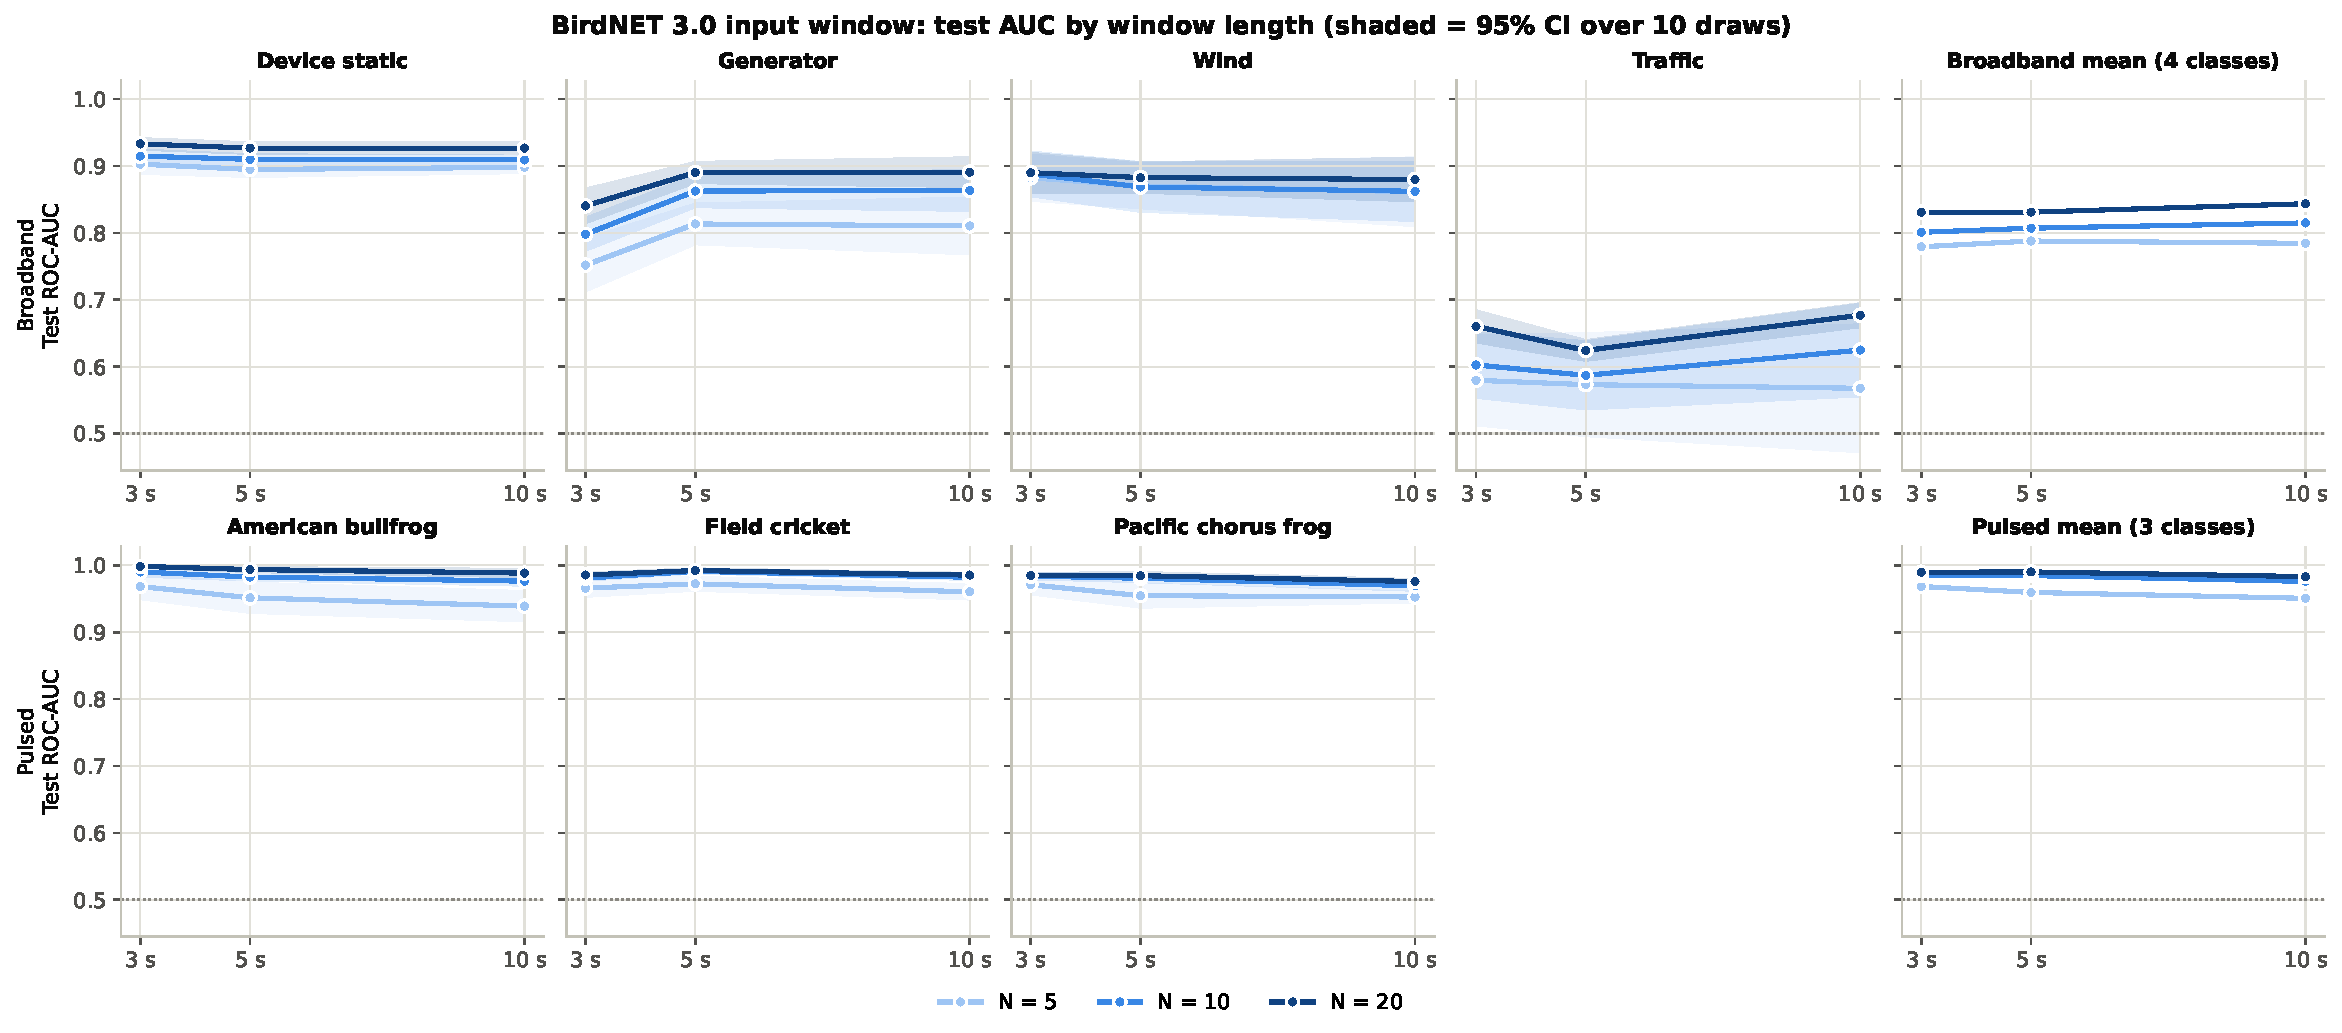
\includegraphics[width=\linewidth,height=0.64\textheight,keepaspectratio]{window_size.pdf}\par\vspace{0.1em}
  {\small At N = 20, generator rises from 0.84 (3 s) to 0.89 (5 and 10 s). Device static and wind are unchanged,
   traffic shows no trend, and pulsed sounds stay at 0.98--0.99.}
\end{frame}

\begin{frame}{Take-home}\framesubtitle{Summary}
  \begin{enumerate}\setlength{\itemsep}{0.45em}
    \item About 40 labelled clips per class brings most classes close to their best performance
    \item The class matters more than the model; more clips from the same few recordings don't help
    \item A trained head usually matches or beats a model's built-in label
    \item Errors fall between acoustically similar sounds, in binary detectors, the multiclass head and the
          embeddings alike
    \item Longer input windows help only generator
  \end{enumerate}
\end{frame}

\begin{frame}[plain]
  \vfill\centering{\color{brand}\LARGE\bfseries Supplementary material}\vfill
\end{frame}

\begin{frame}{Pretrained models}\framesubtitle{Table S1}
  \centering\footnotesize
  \setlength{\tabcolsep}{4pt}\begin{tabular}{lrL{3.4cm}L{4.2cm}}
    \toprule
    Model & Embedding & Input & Built-in labels used for zero-shot \\
    \midrule
    BirdNET 2.4 & 1024-D & 3 s at 48 kHz & Engine, Power tools, Human vocal, Human non-vocal, Gun, Fireworks \\
    BirdNET 3.0 & 1280-D & 3 s at 32 kHz (3, 5 and 10 s in Figure 7) & Human vocal \\
    Perch v8 & 1280-D & 5 s at 32 kHz (padded) & none \\
    Perch 2.0 & 1536-D & 5 s at 32 kHz (padded) & FSD50K classes (Table S2) \\
    CNN14 (AudioSet) & 2048-D & 3 s at 32 kHz & AudioSet classes (Table S2) \\
    ResNet-18 (ImageNet) & 512-D & mel spectrogram, 3 s at 16 kHz & none \\
    \bottomrule
  \end{tabular}
\end{frame}

\begin{frame}{Built-in labels used for zero-shot (direct matches only)}\framesubtitle{Table S2}
  \centering\scriptsize\setlength{\tabcolsep}{3pt}\renewcommand{\arraystretch}{0.95}
  \begin{tabular}{lllL{3.3cm}L{3.3cm}}
    \toprule
    Class & BirdNET 2.4 & BirdNET 3.0 & Perch 2.0 & CNN14 \\
    \midrule
    Device static & & & & Static \\
    Engine & Engine & & Engine; Idling & Engine; Idling \\
    Traffic & & & Traffic noise and roadway noise & Traffic noise, roadway noise \\
    Power tools & Power tools & & Power tool; Drill & Power tool; Drill \\
    Human vocal & Human vocal & Human vocal & Speech; Human voice; Homo sapiens & Speech \\
    Metal clanging & & & & Clang \\
    Airplane & & & Fixed-wing aircraft and airplane & Fixed-wing aircraft, airplane \\
    Gun & Gun & & Gunshot and gunfire & Gunshot, gunfire \\
    Fireworks & Fireworks & & Fireworks & Fireworks \\
    Human non-vocal & Human non-vocal & & & \\
    Wind & & & Wind & Wind; Wind noise (microphone) \\
    Thunder & & & Thunder & Thunder \\
    Water & & & Water & Water \\
    \bottomrule
  \end{tabular}
\end{frame}

\begin{frame}{Clips available for the window-length experiment}\framesubtitle{Table S3}
  \centering
  \begin{tabular}{llr}
    \toprule
    Class & Group & Clips (recordings) \\
    \midrule
    Device static & broadband & 239 (147) \\
    Generator & broadband & 79 (28) \\
    Wind & broadband & 79 (79) \\
    Traffic & broadband & 48 (36) \\
    American bullfrog & pulsed & 378 (13) \\
    Field cricket & pulsed & 539 (103) \\
    Pacific chorus frog & pulsed & 705 (41) \\
    \bottomrule
  \end{tabular}
\end{frame}

\sidefig{Figure S1 \textperiodcentered{} Low-sample classes}{Saturation curves for the low-sample classes (provisional)}
  {saturation_low_sample.pdf}{0.55}{0.42}{%
  \item Test sets of 3--30 clips from 1--13 recordings
  \item Curves end at N = 5--20
  \item The CIs cover training draws only, so they understate test-set uncertainty}

\sidefig{Figure S2 \textperiodcentered{} Head choice}{A linear probe gives the same curves as the MLP head}
  {head_comparison.pdf}{0.68}{0.29}{%
  \item The MLP is ahead by 0.003--0.026 AUC; ranking unchanged
  \item The linear probe is fitted to convergence at every N and shows the same rise with N}

\sidefig{Figure S3 \textperiodcentered{} Cross-detection, all data}{Training on all clips mainly reduces false alarms}
  {cross_detection_all_data.pdf}{0.7}{0.27}{%
  \item False alarms fall from 0.14--0.23 to 0.11--0.17
  \item Recall rises for device static and traffic
  \item No gain for power tools or human vocal (2 recordings each)}

\end{document}
